\chapter{Conceptual Design}
\label{chap:05_design}
%
\todo{Describe Chapter}


% ===========================================
% ===========================================
\section{Design Restrictions}
\label{sec:05_restrictions}
The design of the computing environment will be restricted by several points. These factors are given because of technological choices and requirements from up there.

\begin{itemize}
\item \textbf{Running on a NVIDIA DGX A100\footnote{The Universal System for AI Infrastructure - \url{https://www.nvidia.com/en-us/data-center/dgx-a100/}}:} The environment will run on a NVIDIA DGX A100 workstation. The workstation has 80 CPUs and 8 GPUs installed. For this computing environment, 2 GPUs will be available.

\item \textbf{Apache Spark for distributed computing:} Apache Spark will be used as a distributed computing framework.

\item \textbf{Python as the main programming language:} Python will be used as the main programming language for Apache Spark applications. Therefore, examples will use Python code. Configurations for the system are optimized for using Python in production.

\item GitLab as repository: sadf <- Eher implementation detail/requirement
\end{itemize}

% ===========================================
% ===========================================
\section{Automated Deployment Pipeline}
% Abstract
The objective of this thesis is to automatically submit an Apache Spark application to the Apache Spark cluster to train ML models. Therefore, the training process has to be integrated into the application development lifecycle.
% Git
The source code of an Apache Spark application is hosted on a Git repository. After each committed change on the repository, the pipeline is triggered.


% Conceptual figure
\begin{figure}[h]
\centering
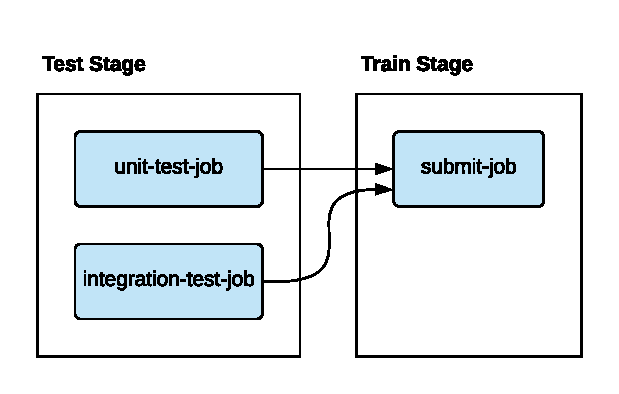
\includegraphics[scale=1]{images/05_conceptual_design/automated_deployment_pipeline/ci_cd_concept}
\caption{Automated Deployment Pipeline concept}
\label{fig:05_deployment_concept}
\end{figure}
% Short intro
\Fig{fig:05_deployment_concept} illustrates the conceptual design of the Automated Deployment Pipeline.
% The stages
The pipeline consists of two different stages:
\begin{enumerate}
\item Test stage: After the build stage has succeeded, the test stage will perform tests.
\item Train stage: If the tests have been successful, the application is submitted to the Apache Spark cluster for training.
\end{enumerate}
% No build stage
It is important to mention, that a build stage is missing in this conceptual design. The build stage includes compiling source code into a format that can be executed directly.
% Python
Python is an interpreted language and therefore no compilation is needed to execute the source code. \todo{Quelle}
% Other languages
As being mentioned in Section SPARK, Apache Spark supports different languages that Python.  For example, for Java application, a build stage is needed to compile the source code to a .jar binary, which can be submitted to the Apache Spark cluster.


\subsection{Test Stage}
% short intro
In order to detect error in an early stage, the source code has to be tested.
% responsibilities
The test stage is responsible to the the source code within a set of various tests. Tests can include:
% Tests
\begin{itemize}
\item Unit tests:
\item Integration tests:
\item End-to-end tests:
\end{itemize}
% Different jobs
For each different test, a new job in the test stage is being created. All jobs will perform in parallel after the test stage has been triggered.
% On failure
If a job has failed, the whole test stage is marked as failure and all participating developers will get a notification.


\subsection{Train Stage}
\paragraph{}
% Short intro
The train stage is responsible to submit the Apache Spark application to the Apache cluster after the test state was successful.
% How
As being mentioned in SECTION XY, an Apache Spark application will be submitted to the Apache Spark cluster by creating a spark-submit Docker container in the same Docker swarm network.
Therefore, after the train stage has been triggered a spark-submit container has to be deployed in the Apache Spark cluster to submit the latest version of the Apache Spark application.

\paragraph{}
% Same machine
To access the Apache Spark cluster Docker swarm network, the train stage has to be executed on the same machine.
% Gitlab runner
Therefore a GitLab runner performing on the machine is needed. Additionally, the GitLab runner needs access to the underlying Docker engine to deploy new container to a given network.
% Perform train stage concept
\begin{figure}[h]
\centering
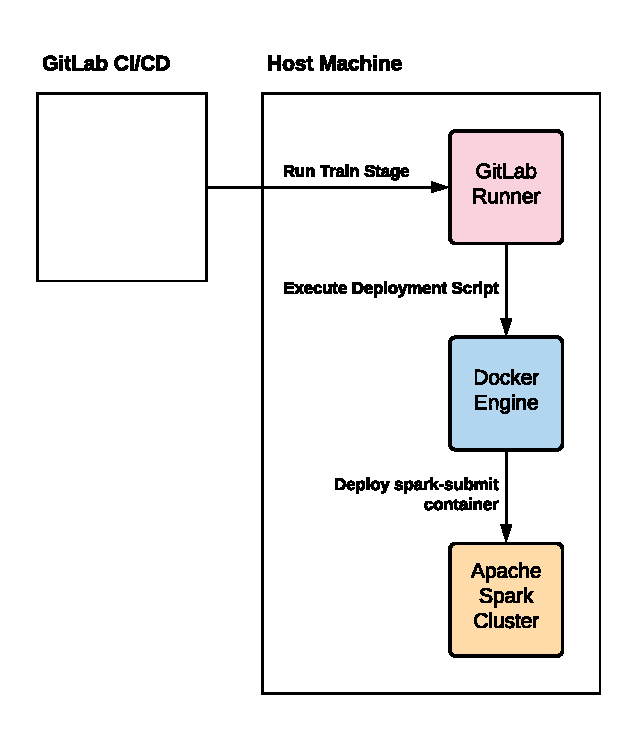
\includegraphics[scale=1]{images/05_conceptual_design/automated_deployment_pipeline/train_stage_runner}
\caption{Deployment of a spark-submit container}
\label{fig:05_deployment_train_concept}
\end{figure}
% Explain figure
\Fig{fig:05_deployment_train_concept} illustrates the steps to deploy a spark-submit container in the Apache Spark cluster swarm network.
% Runner
GitLab CI/CD performs the train stage on the GitLab runner which is running on the NVIDIA DGX machine.
% Deploy
The GitLab Runner executes the deployment script defined in the train stage.
% Deploy script
The deployment script executes Docker CLI commands to deploy a spark-submit container in the Apache Spark cluster swarm network.


% ===========================================
% ===========================================
\section{Identification of Suitable Metrics for Scaling}
% SHort intro
To scale the number of Apache Spark worker in accordance to the actively performing workload, suitable metrics to define the cluster performance have to be defined.
% Rapids enabled GPU
With the RAPIDS accelerator for Apache Spark enabled, the Apache Spark cluster is able to utilize the computing power of GPUs and CPUs to enable parallization.
% SO?
Therefore, suitable metrics to measure the performance are the overall CPU utilization across all worker and the GPU utilization of all available GPUs.
% Those are time-based utilization
These utilization metrics will be based on the time when the Aapche Spark cluster is actively performing computations.


\subsection{CPU Utilization}
% Sharing CPU cores
All Apache Spark worker run on the same machine. Therefore, all available CPU cores on the machine will be shared across each running Apache Spark worker.


% cadvisor
cAdvisor provides a performance called metric \texttt{container\_cpu\_usage\_seconds\_total}\footnote{Monitoring cAdvisor with Prometheus - \url{https://github.com/google/cadvisor/blob/master/docs/storage/prometheus.md} (Accessed: 2021-01-21)}. This metric provides the total amount of CPU seconds consumed by core per container. 
% Overall utilization
To calculate the overall CPU utilization for all Apache Spark worker, the value of the performance metric for each over a specific rate has to be summed up. Therefore, the CPU utilization ($U_{CPU}$) is defined by:

\begin{equation}
U_{CPU}=\sum_{n=1}^{ActiveWorker}container\_cpu\_usage\_seconds\_total_{n}
\label{eq:formel}
\end{equation}

\subsection{GPU Utilization}
% Number of gpus
Two GPUs on the machine are available across all Apache Spark Worker.
% The metric
The dcgm\_exporter agent provides the \texttt{bla\_bla} performance metric. This metric returns the procentual utilization per GPU.
% How to calculate
Therefore, the overall GPU utilization ($U_{GPU}$) is defined by:


The system has a fixed number of GPUs to use.
\begin{equation}
U_{GPU} = \dfrac{\sum bla\_bla}{ActiveGPUs}
\label{eq:formel}
\end{equation}


% ===========================================
% ===========================================
\section{Computing environment Architecture}

\todo{Only self-adapting -> wegen autonomic computing}

\subsection{Overall}
\label{subsec:05_arch_overall}

% Figure
\begin{figure}[h]
\centering
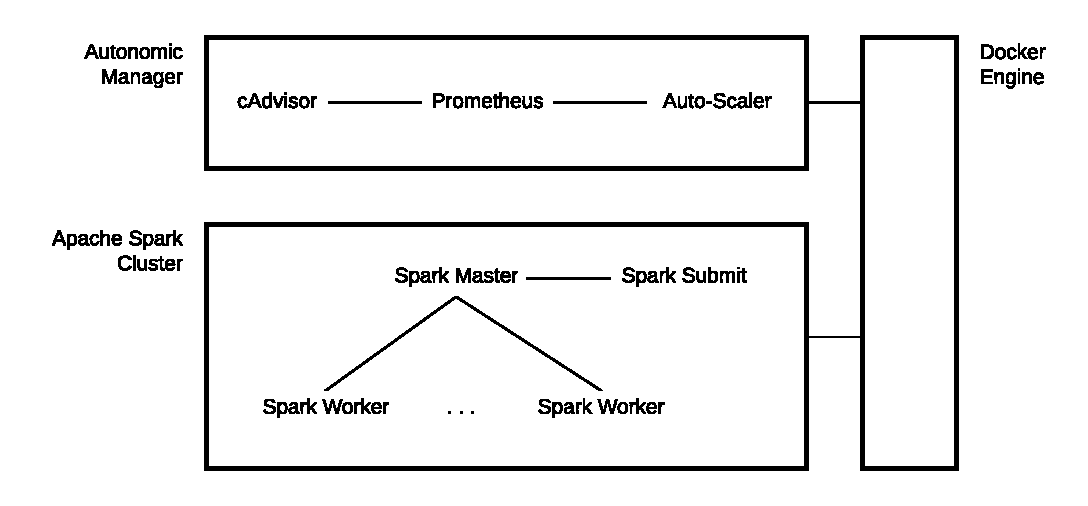
\includegraphics[scale=0.8]{images/05_conceptual_design/cluster_architecture/overall_architecture}
\caption{Overall cluster architecture - Source: Authors own model.}
\label{fig:ca-overall_architecture}
\end{figure}

\Fig{fig:ca-overall_architecture} illustrates the overall architecture with all components of the computing environment. The two main components in the environment are an Apache Spark cluster and an autonomic manager.
% The components
The autonomic manager will be implemented according to the MAPE architecture (introduced in \SubSec{subsec:02_ac_manager}). It is responsible for monitoring and auto-scaling the Apache Spark cluster. To enable distributed computing, an Apache Spark cluster will be set up to execute machine learning applications. 
% The nodes and virtualization
The autonomic manager and the Apache Spark cluster consist each of multiple nodes. Each node of a component will run as a Docker container.
% Self healing
All containers will run as services in Docker Swarm mode. As described in \SubSec{subsec:04_docker_swarm}, Docker Swarm mode will maintain a healthy state of all running containers. Therefore, the environment will enable self-healing according to the requirements of Autonomic Computing described in \Sec{sec:02_ac}.


\subsection{Apache Spark Cluster}
\label{subsec:05_arch_spark}

\todo{Why standalone -> Because most simple way; Master und worker -> Managed Resources}

\subsubsection{Master and Worker}
The Apache Spark cluster will consist of a Spark master node and a dynamic number of Spark worker nodes.
% Master
The Spark master node is responsible to distribute the application workload across available Spark worker nodes.
% Worker
A Spark worker node will execute the workload given by the master node. Each Spark worker is homogeneous. 
% Homegeneous spark worker
Homegenneosity is important to scale the number of worker nodes. To enable homogeneous nodes, each SPark worker node is a Docker container running the same Docker image. In addition, each worker is given the same computing resources. With homogeneous Spark worker nodes, each worker will respond as all other nodes.
% GPU acceleration
To enable GPU acceleration, each WORKER/MASTER will have the RAPIDS plugin installed.
% Standalone mode
The cluster will be deployed in standalone mode. To be able to run Python applications


\subsubsection{Spark Submit}
Because the Apache Spark cluster ill be executed in standalone mode, a node inside the cluster is required to run Spark applications. When a Spark application will be executed, a Spark Submit container will be deployed in the cluster. When the appliccation has finished, the container will be automatically removed.
Each app will be executed by a unique Spark Submit node.
The Spark Submit node will be deployed via the CI pipeline (SECTION XY). The prupose of this 


\subsection{Autonomic Manager}
\label{subsec:05_arch_am}

\begin{figure}[h]
\centering
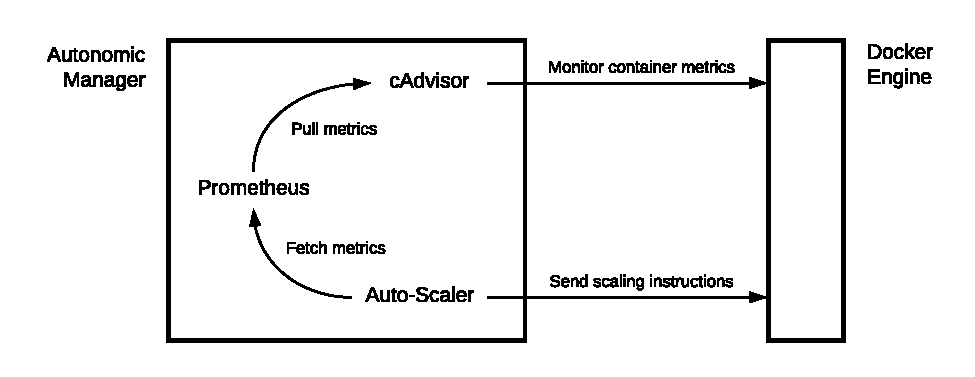
\includegraphics[scale=0.85]{images/05_conceptual_design/autonomic_manager/autonomic_manager_overview}
\caption{Autonomic manager component design - Source: Authors own model.}
\label{fig:am-design-component}
\end{figure}

% MAPE architecture
The design of the autonomic manager needs to fullfill all requirements given by the MAPE architecture (described in \SubSec{subsec:02_ac_manager}). It will be responsible to monitor the performance of Apache Spark worker nodes in the environment, analyze the metrics and plan and execute scaling actions in accordance to fullfill the performance goals.
% Figure
As illustrated in \Fig{fig:am-design-component}, the autonomic manager consists of a cAdvisor, Prometheus and Auto-Scaler node. Together, all three nodes build a complete autonomic manager in accordance to the MAPE architecture. Each node will run as a Docker container.
% Explain figure
For monitoring, cAdvisor collects metrics from all available Docker container in the computing environment. Prometheus pulls metrics from cAdvsior. The Auto-Scaler will fetch metrics from Prometheus and send scaling instructions to the Docker engine.


\subsubsection{Monitoring System}
% Why - dynamic env, requirements, etc
The design introduced in \SubSec{subsec:05_arch_overall} is a dynamic changing computing environment. To monitor this dynamic environment, a monitoring-system is needed that fullfills the requirements described in \Sec{sec:02_monitoring}.


% Gathering metrics
cAdvisors will be used as an agent to collect performance metrics from all running Docker containers in the environment.
% Store metrics
Prometheus pulls the collected performance metrics from cAdvisor and stores the data as time-series data in its database.
% Query
In addition, Prometheus provides a powerful multi-dimensional query language to aggregate and analyze the stored data.

% Collecting operational data can be challenging in a horizontally        scaling environment since the number of nodes varies over time. Any        system that automates gathering of log files from individual nodes        needs to account for this, and care needs to be taken to ensure that        logs are captured before nodes are released.


\subsubsection{Workflow}

\paragraph{} The workflow of the autonomic manager is implemented as a loop.

% Workflow
\begin{figure}[h]
\centering
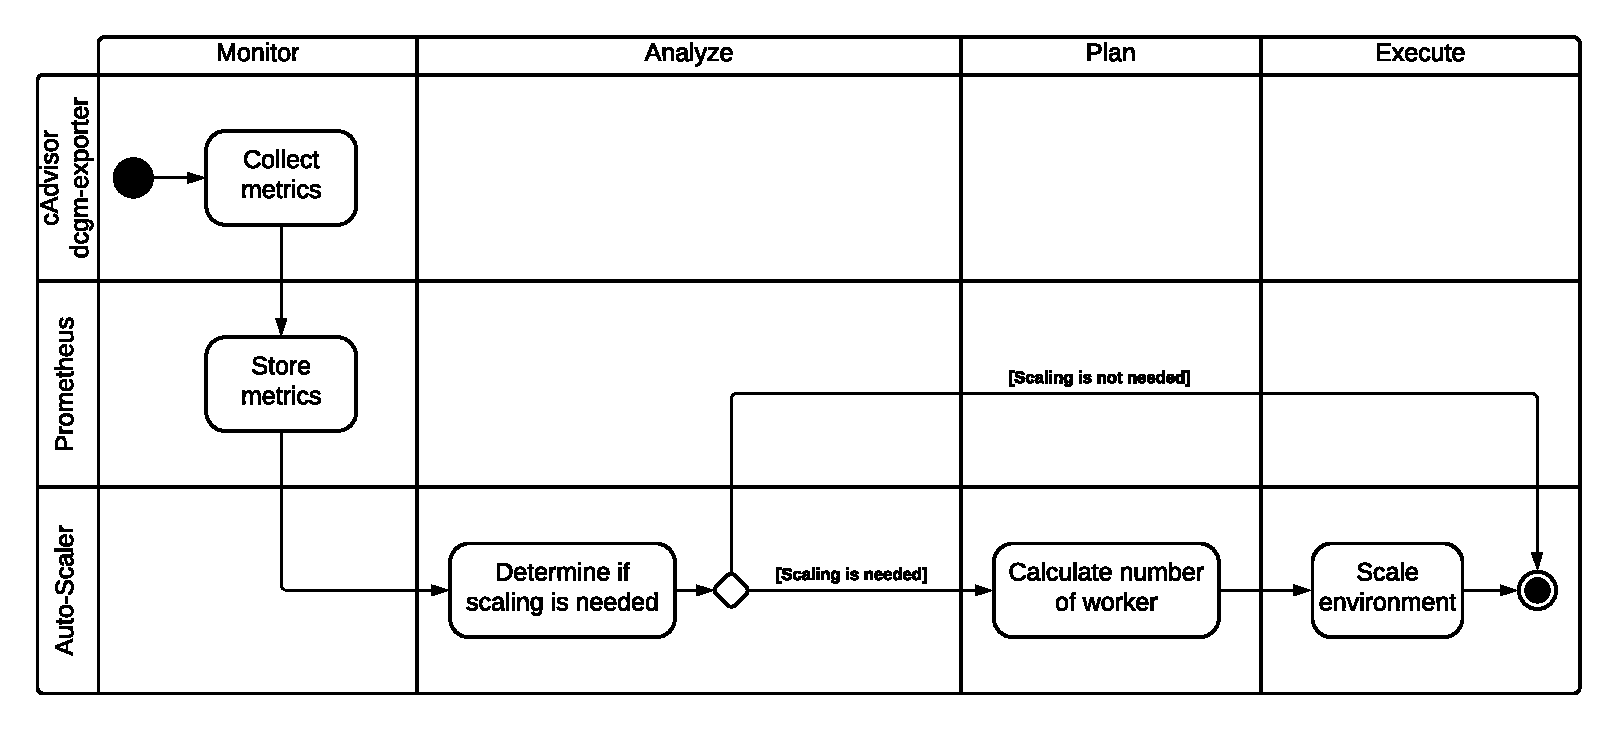
\includegraphics[scale=0.50]{images/05_conceptual_design/autonomic_manager/autonomic_manager_workflow}
\caption{UML activity model of the autonomic manager process - Source: Authors own model.}
\label{fig:am-workflow}
\end{figure}
% Explain figure
\paragraph{} \Fig{fig:am-workflow} illustrates all steps of each component of the autonomic manager process according to the MAPE architecture.


% Monitor
The workflow starts with collecting metrics in the monitor phase. cAdvisor is responsible to collect metrics from the Docker engine. After that, Prometheus stores the collected metrics as time-series data in its database.
% Analyze
Next, in the analyze phase, the Auto-Scaler needs to determine if a scaling action is needed. If scaling the Apache Spark worker nodes is not needed, the process has finished and will repeat from the beginning in the next period.
% Plan
If the performance is over- or under-utilized, a scaling action is needed. Then, the Auto-Scaler needs to determine how many Apache Spark worker nodes are needed to reach the performance goal.
% Execute
Lastly, the Auto-Scaler is responsible to send the scaling instructions to the Docker engine.


% ===========================================
% ===========================================
\section{Auto-Scaler}
\label{sec:05_auto-scaler}
% What is the Auto-Scaler
The Auto-Scaler is a component of the the Autonomic Manager and is responsible for the analyze, plan and execution phase.
% Complete autonomic manager
Together with cAdvisor and Prometheus, the Auto-Scaler builds a complete Autonomic Manager according to \SubSec{subsec:02_ac_manager}.
% control loop
In addition, the Auto-Scaler implements the control-loop which is responsible to make adjustments in the environment according to the performance.
% Communication with Prometheus
To adjust the number of Apache Spark worker in the environment, the Auto-Scaler needs to perform queries on the performance metrics stored in Prometheus.
% Analyzing
After analyzing the performance metrics, the Auto-Scaler will send instructions to adjust the number of Apache Spark worker to the Docker engine. The Docker engine tells the Swarm manager to scale the replicas of the Apache Spark service in accordance to the Auto-Scaler instructions.

\todo{HIER NOCH BILD VON SCALER WIE MIT DER MAPE ARCH; Reactive Auto-Scaler, threshold-based rules}


\subsection{Configuration}
\label{subsec:05_auto-scaler_configuration}
The Auto-Scaler needs specific configuration properties to be able to collect the correct metrics from Prometheus and deploy new Apache Spark worker container in the environment. The following are properties that have to be defined to ensure that the Auto-Scaler is able to collect meaningful metrics and scale Apache Spark worker as expected.

\subsubsection{General properties}

\begin{itemize}
\item \textbf{Interval seconds:} The number of seconds when the loop has to repeat needs to be defined.

\item \textbf{Cooldown period:} The duration in seconds,  the Auto-Scaler has to wait after a scaling action was performed.

\item \textbf{Recurrence factor:} To prevent to many scaling actions,  the autonomic manager should only execute a scaling action,  if the utilization thresholds is violated \textit{n} times.

\item \textbf{Prometheus URL:} The Auto-Scaler will fetch the configured metrics from the Prometheus REST API.
\end{itemize}

\subsubsection{Metrics}

To support to analyze multiple metrics, the user should be able to create a dynamic list if metrics. Each metric needs to have a variety of properties configured.

\begin{itemize}
\item \textbf{Target utilization:} The relative target utilization of a metrics needs to be defined to calculate the number of Spark worker to add or to remove to reach the defined goal.

\item \textbf{Utilization thresholds:} To determine if a scaling action is needed, the scaling heat algorithm needs the minimum and maximum utilization defined by an administrator.

\item \textbf{Query:} A PromQL query needs to be defined to collect the metric for all Spark Worker.
\end{itemize}

\subsubsection{Apache Spark worker properties}

\begin{itemize}
\item \textbf{Worker image:} To guarantee that each Spark worker is homogeneous, all worker container should be created with the same image.

\item \textbf{Worker network:} To establish communication between all Spark worker and the Spark master, all new Spark worker container should be in the same network.

\item \textbf{Worker thresholds:} The minimum and maximum number of concurrent Spark worker should be defined. To avoid the cold start effect, the minimum amount of worker should be 1. 

\item \textbf{Apache Spark master URI:} To distribute the workload across all Spark Worker, all Spark Worker need to communicate with the Spark master.
\end{itemize}


\subsection{Analyze}
% Short intro to analyze phase
In order to determine if a scaling-action is necessary, the Auto-Scaler has to process the collected metrics. 
% How to analyze
During each period, the Auto-scaler queries the Prometheus time-series database with the configured queries to get all needed metrics. 
% Determine if scaling is needed
After the metrics are received, the Auto-Scaler determines if a scaling action is needed using the Scaling Heat algorithm (introduced in Section AB). If scaling is not necessary, the Auto-Scaler continues to collect metrics from Prometheus.


\subsection{Plan}
% Short intro
If a scaling-action is necessary, the Auto-Scaler is responsible to plan how to scale the number of Spark worker to satisfy the defined utilization goals.
% What is a scaling plan
A scaling plan consists of instructions to add or remove Spark worker which will be send to the Docker engine.
% Calculating Spark worker
To calculate the number of Spark worker, needed to accomplish the defined target utilization, the Auto-Scaler uses the \textit{Kubernetes Horizontal Pod Auto-Scaling} algorithm. In addition, the Auto-Scaler needs to check if the estimated number of Spark worker fall bellow the minimum threshold or exceed the maximum threshold of concurrent Spark worker.


\subsection{Execute}
% Short intro
After a scaling plan has been created, the Auto-Scaler needs to send the instructions to the Docker engine.
% Cooldown
After scaling the environment, it needs time for changes to take effect. Therefore a cooldown period will be activated after each scaling action.
% Whats happens
During the cooldown period, no scaling actions will be forwarded to the Docker engine.
